\documentclass[fontsize=10pt,paper=a4,bibliography=totoc]{scrartcl}

%\usepackage[utf8]{inputenc}
%\usepackage[ngerman]{babel}
%\usepackage{amsmath}
%\usepackage{graphicx}
%\usepackage{units}

% packages  
\usepackage[utf8]{inputenc}
\usepackage[T1]{fontenc}
\usepackage{ae}
\usepackage{tabularx}
\usepackage{amsmath,amssymb}
\usepackage[pdftex]{graphicx}
\usepackage{subfigure}
\usepackage{url}
\usepackage[T1]{fontenc}
\usepackage{ifthen}
\usepackage{hyperref}
\usepackage[absolute,overlay]{textpos}
\usepackage{tikz}
\usepackage[ngerman]{babel}
\usepackage{units}

\graphicspath{{images/}}

\definecolor{darkgreen}{rgb}{0,.5,0}

\newcommand{\kai}[1]{{ \color{red} #1 }}
\newcommand{\felix}[1]{{ \color{darkgreen} #1}}
\newcommand{\maxim}[1]{{ \color{blue} #1}}

\newcommand{\todo}[1]{{\color{magenta}#1}}


\usepackage{url}
\title{Ausarbeitung\\Solarthermisches Kraftwerk}

\author{K. Franke, M. Dolgov, F. Achilles\\The Raymen}
\begin{document}
\maketitle
%
\kai{Kai, du schreibst ab jetzt rot.}\newline
\felix{Felix, du schreibst ab jetzt grün.}\newline
\maxim{Maxim, du schreibst ab jetzt blau.}\newline

\section{Stand der Technik}

\subsection{Dish-Stirling Anlage}
Die Dish-Stirling Anlage besteht aus einem großen Parabolspiegel, der meistens aus mehreren kleinen Spiegeln zusammengesetzt wird. Im Brennpunkt befindet sich ein Stirling Motor, der aus der gebündelten Wärme Strom erzeugt. Damit die Strahlen sich immer im Brennpunkt treffen, wird der große Parabolspiegel mit der Sonne mitgedreht um immer senkrecht einfallende Strahlen zu erreichen. Für dieses Konzept ist somit immer eine zweiachsige Nachführung des Spiegels nötig, da nicht senkrecht einfallende Strahlen den Absorber des Stirling Motors verfehlen würden. Dieses Konzept funktioniert daher nur bei direkter Sonneneinstrahlung und nicht bei diffusem Licht. Bild einfügen! Vorteil dieses Kraftwerktyps ist die sehr kompakte Bauweise, so können diese Kraftwerke schon für Leistungen ab ??
%TODO Finden
 kW eingesetzt werden. Nachteil ist die Skalierbarkeit. So kann die Spiegelgröße zwar nach der geforderten Leistung und der Sonneneinstrahlung am Standort gewählt werden, dies ist konstruktionsbedingt aber nur bis zu einer gewissen Größe möglich, da die Windlasten des Spiegels immer größer werden. Besonders die Nachführung wird bei steigender Spiegelgröße immer größer und damit teurer.
 
\subsection{Parabolrinnenkraftwerk}

\maxim{Vielleicht besser: Bei Parabolrinnenkraftwerken wird das einfallende Sonnenlicht von gewölbten Spiegeln auf eine Linie fokussiert. Ein mit Öl gefülltes Absorberrohr verläuft entlang dieser Linie. Die durch das Öl transportierte Energie kann in einem Gas- oder einem Dampfkraftwerk zur Stromerzeugung genutzt werden (s. Abb~\ref{pic:parabolrinnen}). Der Vorteil von Parabolrinnenkraftwerken gegenüber Dish-Stirling-Anlagen besteht darin, dass die Nachführung nur
%http://upload.wikimedia.org/wikipedia/commons/6/63/Solar_Plant_kl.jpg 
\begin{figure}[h]
	\centering
	\def\svgwidth{.6\textwidth}
	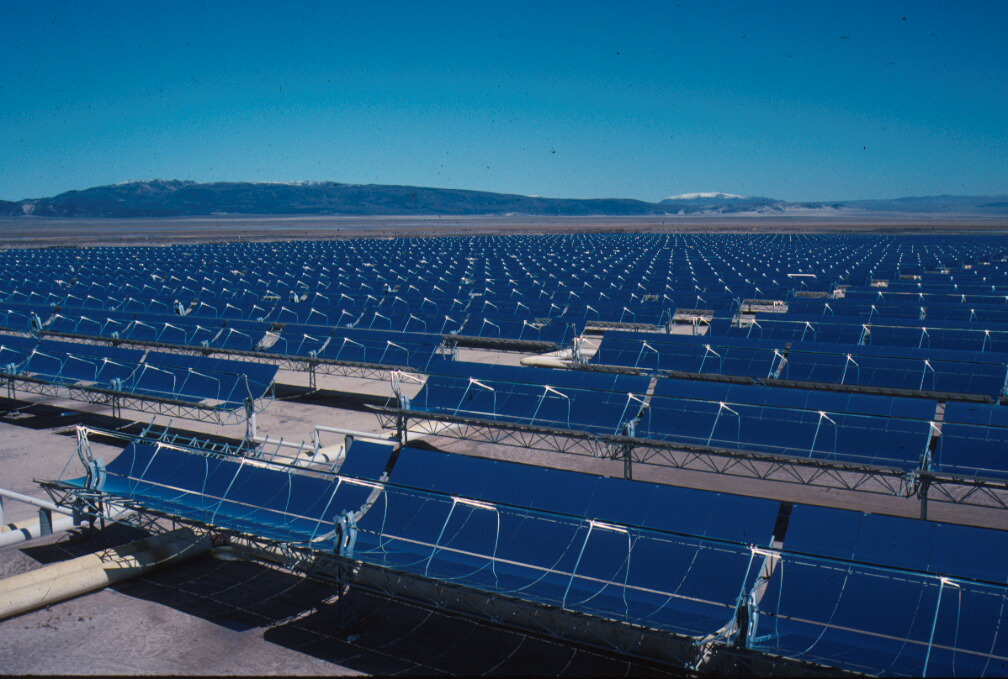
\includegraphics[width=\textwidth]{Solar_Plant_kl}%felix
	
	%\input{images/Parabolrinnenkraftwerk.pdf_tex}
	\label{pic:parabolrinnen}
\end{figure}
}\hfill\newline\newline
\kai{gekauft, allerdings solltest du Parabolrinnenkraftwerk.$pdf_tex$ noch hochladen}

\felix{was ist das denn für ne Bildendung $pdf_tex? ;-)$}

Das Parabolrinnenkraftwerk fokussiert die einfallenden Strahlen nicht auf einen Punkt, sondern auf eine meist mit Öl gefüllte, im Brennpunkt liegende Röhre. Da es sich hier nicht um einen Punktabsorber, sondern um einen in eine Dimension ausgebreiteten Absorber handelt, ist auch nur eine eindimensionale Nachführung nötig. Das erhitzte Öl kann anschließend über Wärmetauscher in einem Gas und Dampfkraftwerk Strom erzeugen. Bild einfügen! Vorteil dieser Technik im Vergleich zur Dish-Stirling Anlage ist, dass eine einachsige Nachführung günstiger ist und das System sehr gut skaliert. Außerdem ist durch ein stationäres Kraftwerk ein besserer Wirkungsgrad erreichbar als durch einen Stirlingmotor
%TODO Nachweis für Wirkungsgrad
 (Nachweis einfügen, wer findet einen?). In großen Solarthermiekraftwerken werden daher meistens Parabolrinnen eingesetzt. Nachteil ist, dass hier eine größere Fläche nötig ist, damit sich der Bau eines stationären Kraftwerks lohnt.

\emph{Gesamtwirkungsgrad hinzufügen wenn ihn jemand findet, vielleicht auch rauslassen, wenn wir den Gesamtwirkungsgrad von unserem Kraftwerk nicht berechnen können.}

\section{Idee}


\maxim{
Die Hauptidee unseres Konzepts besteht darin die kompakte Bauweise einer Dish-Stirling-Anlage und die Skalierbarkeit sowie stationäre Stromerzeugung eines Parabolrinnenkraftwerks zu kombinieren. Die Anlage soll dabei aus einem großen, fest montierten Hauptspiegel sowie einem auf einer Schiene beweglichen kleineren Zweitspiegel bestehen,} \felix{ was in Abbildung~\ref{pic:system_rendered} veranschaulicht wird.}

\begin{figure}[htb]
	\centering
	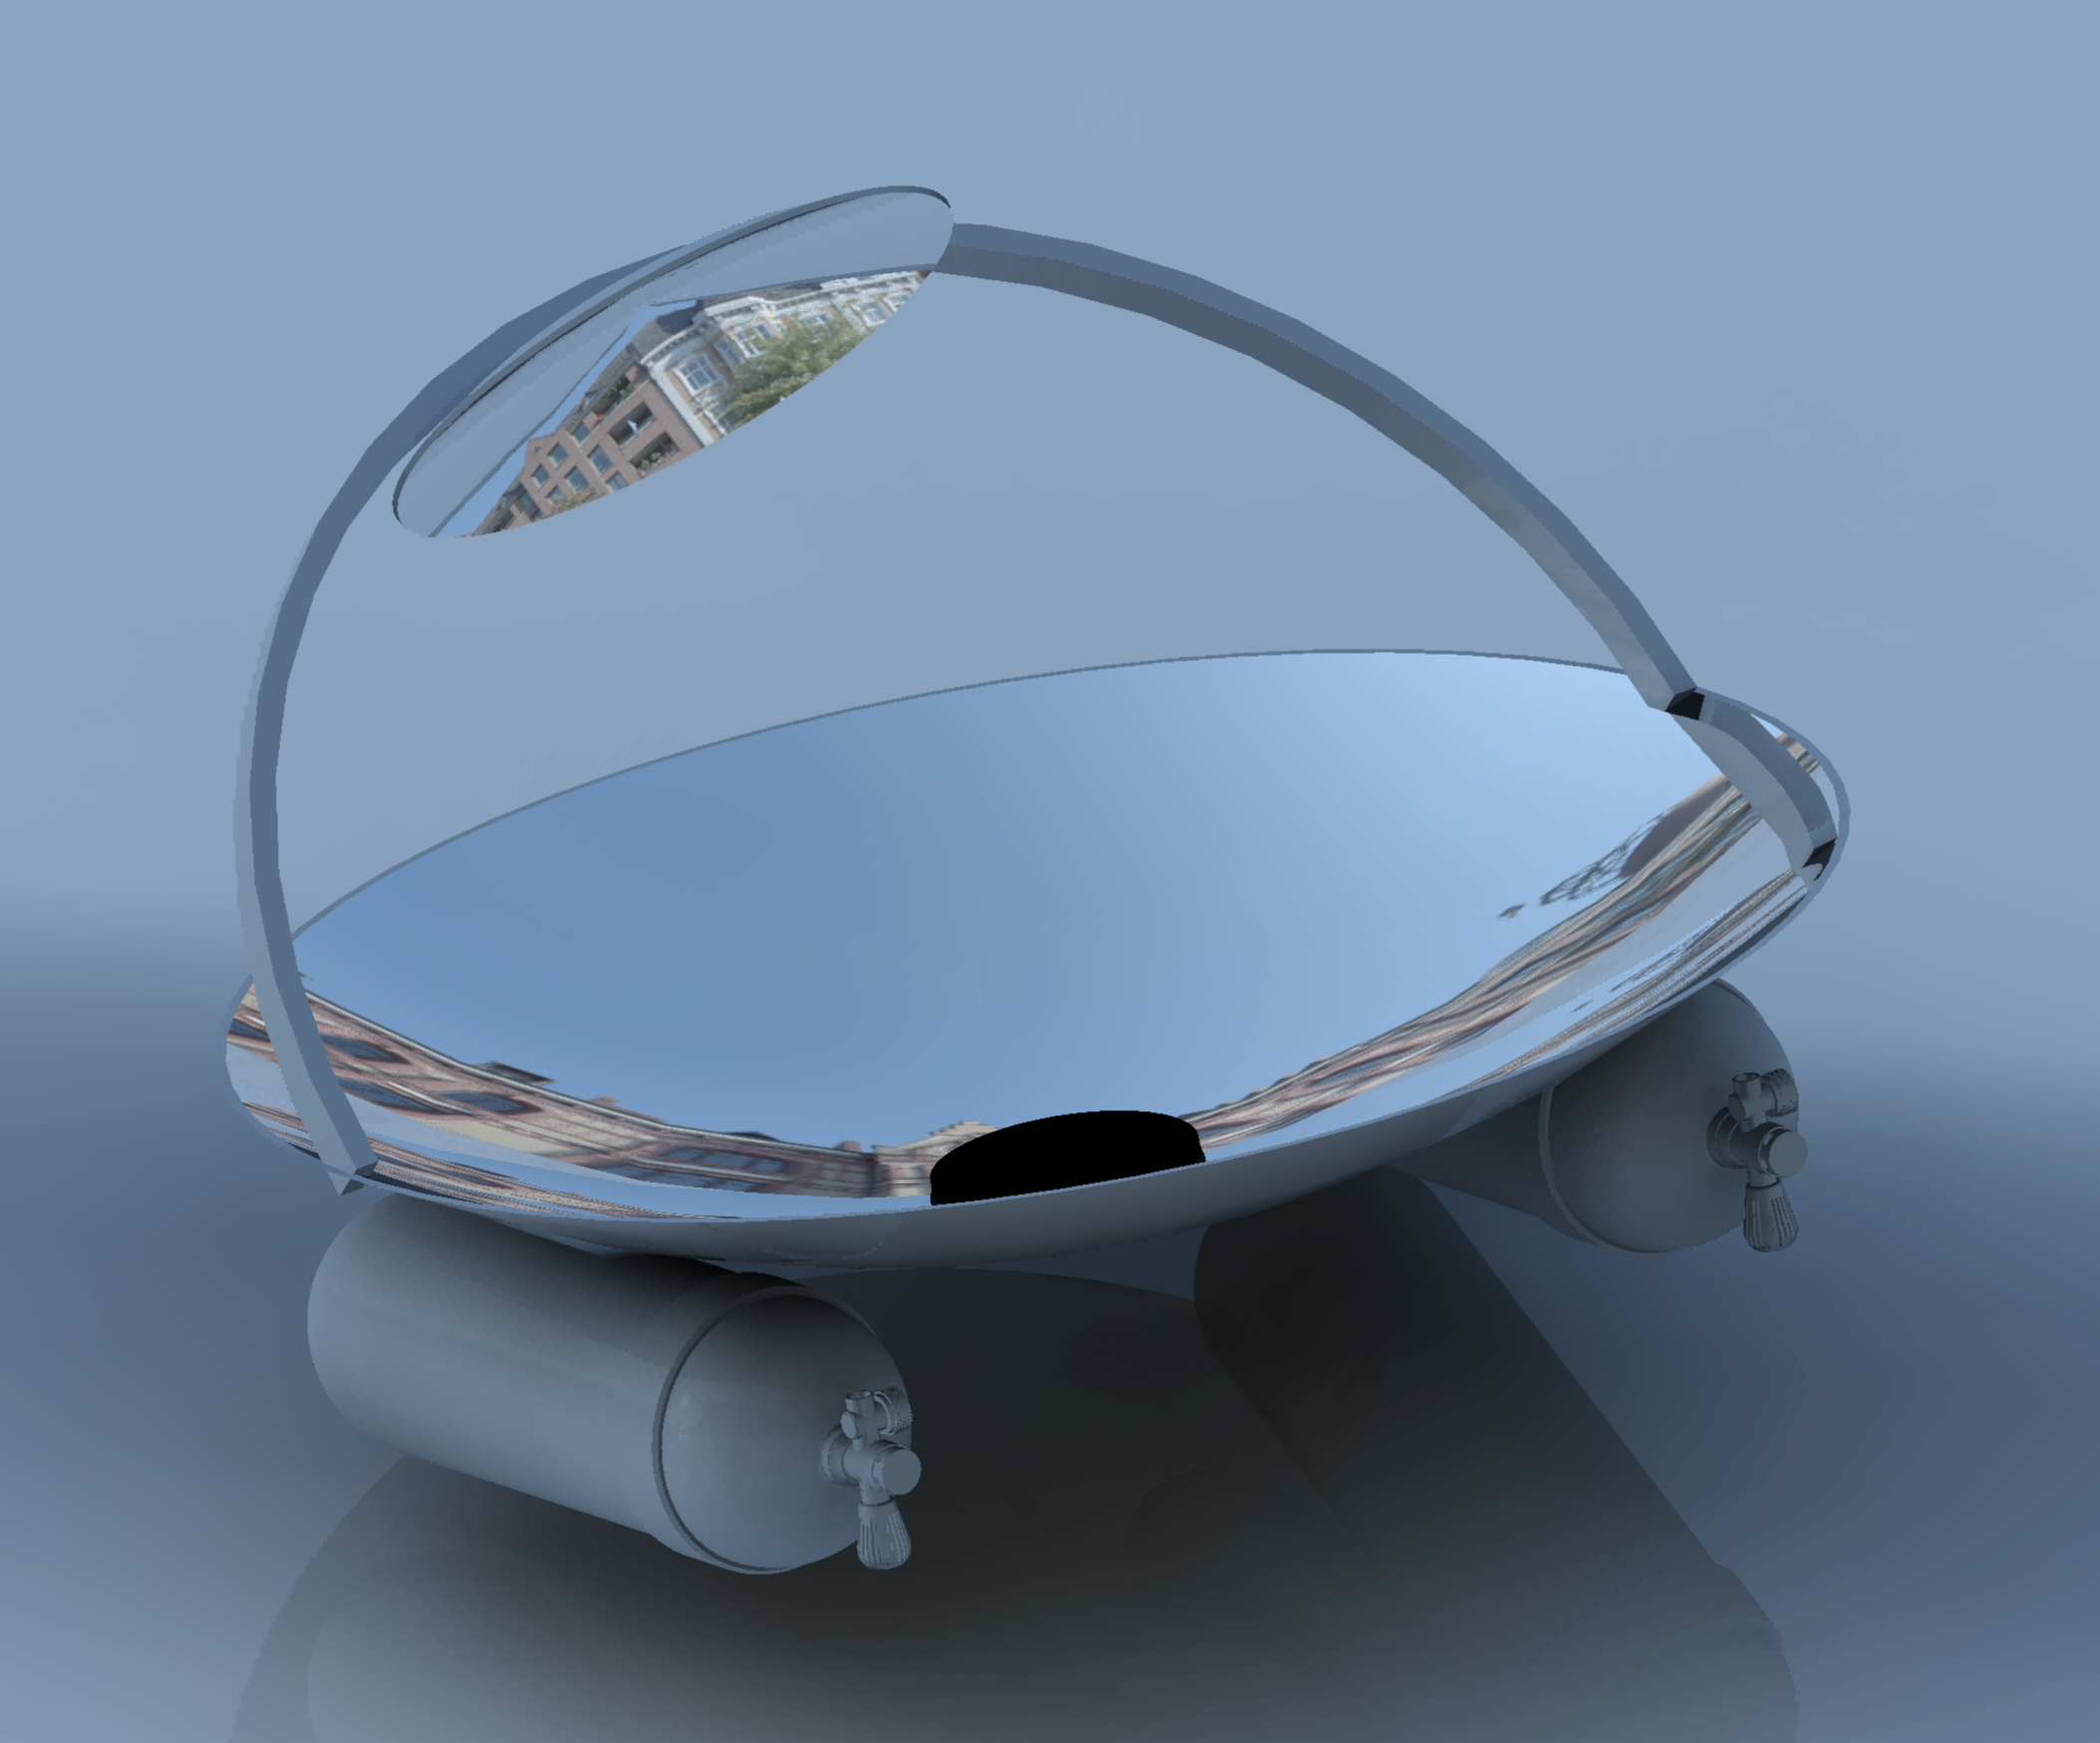
\includegraphics[width=\textwidth]{images/SMALL_MIRROR}
	\caption[Gesamtsystem]{Gesamtsystem mit großem und kleinen Spiegel, schwenkbarer Führungsschiene und Absorber.}
	\label{pic:system_rendered}
\end{figure}

%\todo{Bild}
\maxim{Das einfallende Sonnenlicht wird zunächst vom Hauptspiegel reflektiert. Der Zweitspiegel folgt stets dem Fokuspunkt des Hauptspiegels, welcher seine Position abhängig von der Tages- und Jahreszeit verändert, und reflektiert das Licht anschließend zu einem in den Hauptspiegel integrierten Absorber.  Die im Absorber gesammelte Energie wird zur Stromerzeugung in einem stationären Kraftwerk verwendet.
\hfill\newline %felix: wozu braucht man egtl das hfill hier?
\hfill\newline
Neben geschildertem Aufbau des Kraftwerks, wird ein Konzept zur Energiespeicherung in einem Luftdrucksystem vorgestellt, welches vor allem für Privathaushalte eine On-Demand-Stromerzeugung ermöglichen soll.
}
\hfill \newline

Ziel dieses Projekts ist die Kombination der kompakten Bauweise einer Dish-Stirling Anlage und der guten Skalierbarkeit des Parabolrinnenkraftwerks mit ein stationären Kraftwerk. Da das Kraftwerk für den Standort Karlsruhe entwickelt werden soll, ist auch zu bedenken, dass hier auch sehr viel diffuse Sonnenstrahlung vorhanden ist, die nach Möglichkeit genutzt werden sollte. Aufgrund der kleinen Abmessungen von nur $10\unit{m}^3$ kam nur eine zweidimensionale Nachführung in Kombination mit einem großen Parabolspiegel in Frage, dabei sollte aber der große Spiegel wegen der Windlasten und einer deutlich einfacheren Konstruktion nicht nachgeführt werden. Stattdessen wurde ein zweiter, deutlich kleinerer Spiegel hinzugefügt, der zweiachsig auf einer Schiene nachgeführt wird und immer im Fokuspunkt der Strahlen steht. Dieser Spiegel reflektiert die eingefangenen Strahlen wieder zurück auf die Mitte des großen Spiegels wo der Absorber platziert ist. Das einzig bewegliche Teil ist also ein leichter Spiegel, der auf einer Schiene fährt. Der Absorber kann wie im Fall des Parabolrinnenkraftwerks an ein stationäres Kraftwerk gekoppelt werden, es entfällt aber der Transport des Öls. Da sich ein Gas und Dampfkraftwerk bei der gegebenen Grundfläche nicht rentiert, wird ein alternatives Konzept vorgeschlagen, das durch die Erwärmung von Luft eine Druckdifferenz erzeugt, die über einen Luftdruckmotor in elektrischen Strom gewandelt werden kann.


\section{Vorstellung des Konzepts}
Es wurde zuerst untersucht wie sich schräg einfallende Strahlung auf den Fokuspunkt der Strahlen auswirkt. Für solche Versuche wurde ein Raytracing Programm in Matlab geschrieben, das beliebig viele Strahlen in einer beliebigen Richtung erzeugt, den Schnittpunkt mit einem Spiegel findet, die Reflexionsrichtung berechnet und alles grafisch darstellen kann. Das Ergebnis ist in Abbildung~\ref{pic:2dreflektion} zu sehen. Während die Strahlen bei senkrechtem Lichteinfall genau im Fokuspunkt gebündelt werden, verschiebt sich dieser
bei schrägem Einfall%hat gefehlt ;)
nicht nur, die Strahlen werden nun auch nicht mehr so gut gebündelt, sondern fächern auf (siehe Abbildung~\ref{pic:2dreflektion_schraeg}). 

\begin{figure}[ht]
	\centering
	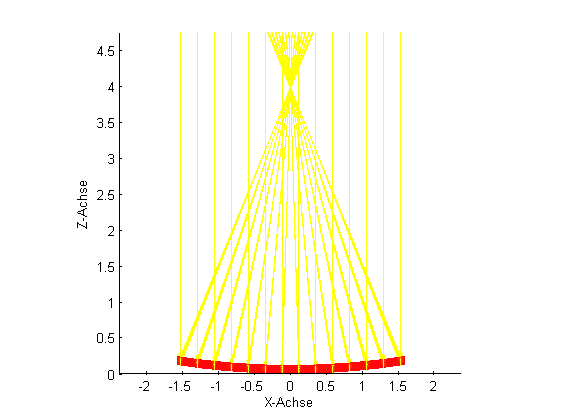
\includegraphics[width=\textwidth]{images/2d_gerade}
	\caption{Gerader Einfall auf Parabolspiegel}
	\label{pic:2dreflektion}
\end{figure}
\begin{figure}[ht]
	\centering
	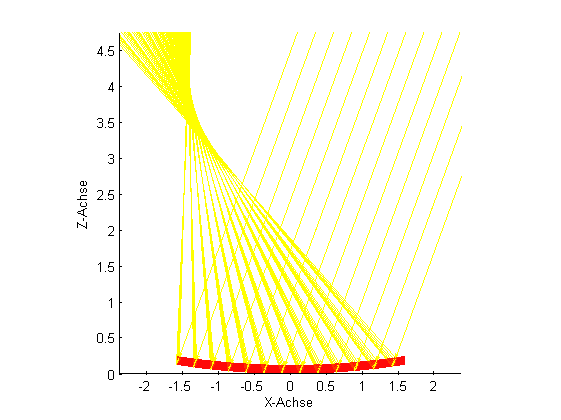
\includegraphics[width=\textwidth]{images/2d_schraeg_20_grad}
	\caption{Schräger Einfall auf Parabolspiegel (20$^{\circ}$ zur vertikalen Achse)}
	\label{pic:2dreflektion_schraeg}
\end{figure}

\subsection{Erhoffte Vorteile}

\section{Beschreibung des Programms}
\maxim{
Zur Berechnung der Geometrie des beschriebenen Zweispiegelsystems wurde ein Mat"-lab-Programm geschrieben. Dieses Berechnet die optimalen Formen der Spiegel durch Lösen eines Maximierungsproblems, welches darin besteht, eine möglichst große Strahlendichte pro Absorberfläche zu erhalten. Die } \felix{Die what? $:-P$}\maxim{
Nachfolgend wird die Vorgehensweise des Programms grob beschrieben.
}

\felix{
\subsection*{Kollisionsdetektion}
Eine Kollision von Strahlen und Spiegelfläche muss zu vier Zeitpunkten des Programms überprüft werden:
\begin{enumerate}
\item Reflektion am großen Spiegel,
\item Reflektion am kleinen Spiegel (blockierende Rückseite),
\item Reflektion am kleinen Spiegel (spiegelnde Vorderseite),
\item Absorption in der Absorberfläche.
\end{enumerate}
Dabei wird jedes Mal auf dasselbe Subprogramm zugegriffen. Dieser "Dychotome Collision Tracker" benötigt einen Ausdruck einer Spiegelfunktion in der Form $Z = f(X,Y)$, sowie ein Array, in dem die Strahlen (Startpunkt, Richtung) gespeichert sind.


Der Collision Tracker folgt zunächst der Richtung jedes Strahls in einer festgelegten Schrittweite. Sobald eine Höhe $Z_{unter}$ erreicht wird, die kleiner als die Spiegelhöhe $Z_{Spiegel}$ an diesen Koordinaten ist, weiß man, dass man den Spiegel durchstoßen hat.


Darauf beginnt die zweite Art der Suche, bei der der Suchraum mit jedem Schritt halbiert wird. Diese Dychotome Suche vergleicht, ob die Mitte zwischen zwei Randpunkten über oder unter dem Spiegel liegt. Ein Randpunkt ist dabei der soeben erreichte $Z_{unter}$, der zweite ist der Punkt $Z_{ueber}$, der vor dem Durchstoßen erreicht wurde. Zwischen diesen beiden Grenzen muss zwangsweise der genaue Kollisionspunkt liegen. Liegt die Mitte mit der Höhe $Z_{Mitte} = \dfrac{Z_{ueber} + Z_{unter}}{2}$ oberhalb des Spiegels an diesen Koordianten, so wird die Mitte die neue obere Grenze: $Z^{\ast}_{ueber} := Z_{Mitte}$. Andersherum wird die Mitte zur neuen unteren Grenze, wenn sie unterhalb des Spiegels liegt. Darauf wiederholt sich die Berechnung des Mittelpunkts und dessen Vergleich mit der Spiegelhöhe. Ist eine vorgegebene Genauigkeit des Unsicherheitsintervalls erreicht, terminiert der Algorithmus und gibt den aktuellen Mittelpunkt als Kollisionspunkt aus.
}
\subsection{Ablaufdiagramm (Top-Level)}
\maxim{

}
\subsection{Möglichkeiten und Grenzen}
 (versch. Breitengrade, über ein Jahr hinweg etc.)
\section{Gesamtaufbau}
\subsection{CAD-Modell mit allen Nebenaggregaten}
 (Antriebe: Stirling, Turbine)
\subsection{Verschiedene Generatorantriebe}
 (Stirling, Turbine)
\section{Kosten}

\section{Ergebnisse}
\felix{
Bis zu diesem Zeitpunkt (\today) haben wir einige Szenarien der Optimierung durchgerechnet. Die grundlegende korrekte Funktion des Raytracers soll in Abbildung~\ref{pic:netteReflektion} verdeutlicht werden. Nur Sonnenstrahlen, die den blau dargestellten Absorber treffen, sind abgebildet. Der große und kleine Spiegel haben jeweils Parabolform , dabei wird die Grundfläche des großen Spiegels von den vorgegebenen \unit[10]{m$^2$} begrenzt.

\begin{figure}[htb]
	\centering
	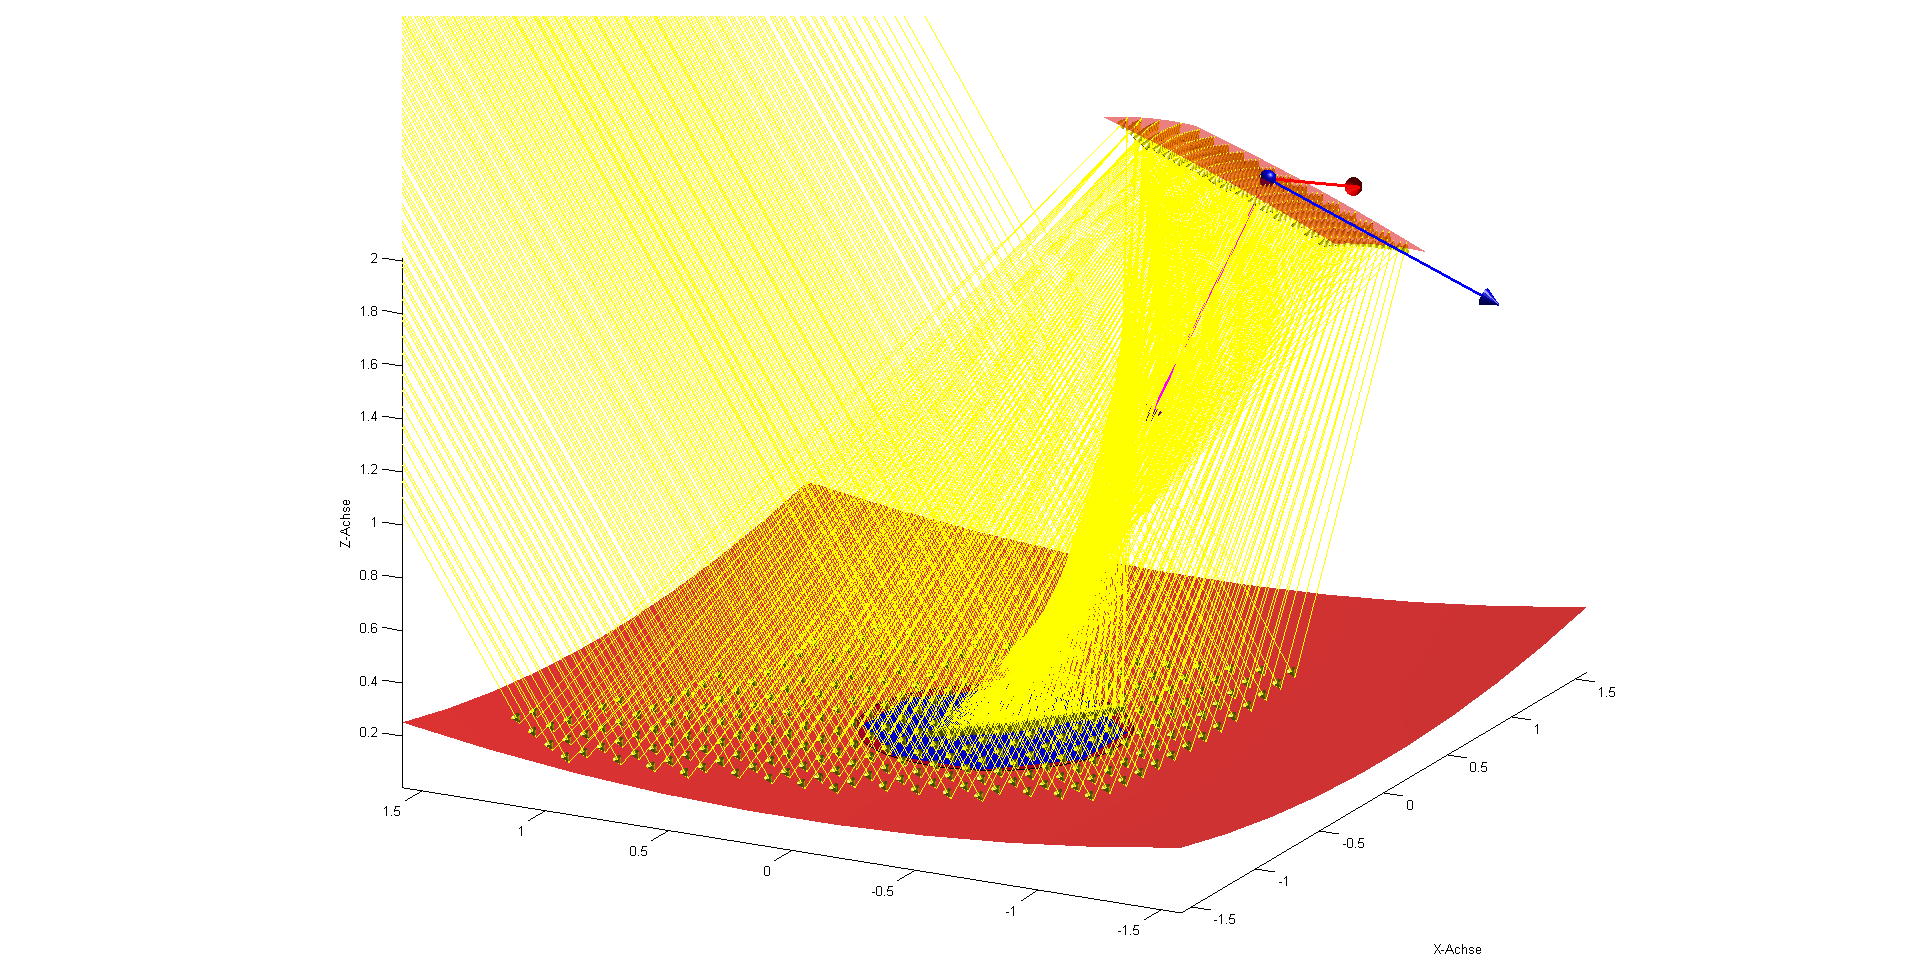
\includegraphics[width=\textwidth]{images/netteReflektion}
	\caption[Bündelung schräg]{Schräger Einfall auf Parabolspiegel, Reflektion und Bündelung durch zweiten kleineren Spiegel.}
	\label{pic:netteReflektion}
\end{figure}

Zu erkennen ist die korrekte Verschiebung des kleinen Spiegels an den Ort des verschobenen Fokuspunktes (vgl. Abb.~\ref{pic:2dreflektion_schraeg}), sowie dessen Ausrichtung auf den Absorber.

Ungefähr \unit[40]{\%} der zur Verfügung stehenden großen Spiegelfläche werden von Strahlen getroffen, die den Absorber erreichen. Dies entspräche also einem Wirkungsgrad $\eta_{Sonne}$ von \unit[40]{\%}. Für eine Abschätzung des Gesamtwirkungsgrades $\eta_{gesamt}$ muss noch der Wirkungsgrad des nachgeschalteten Generators multipliziert werden.
}
\section{Alles Mögliche}

\begin{align*}
	AirMass(\xi)=\frac{1}{\cos(\xi)}
\end{align*}

\begin{figure}[htb]
	\centering
	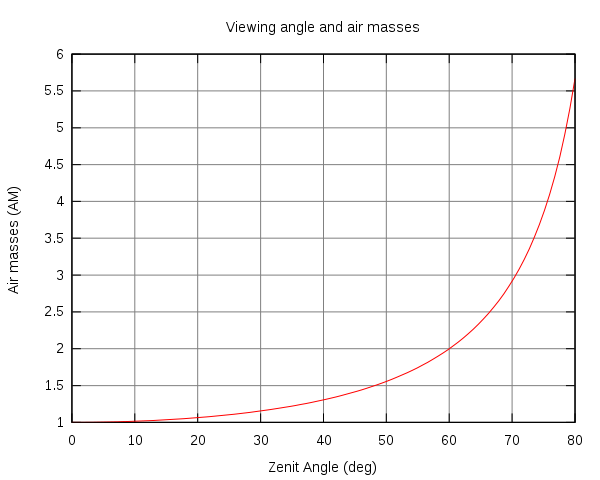
\includegraphics[width=\textwidth]{images/Airmass.png}
	\caption{Luftmasse in Abhängigkeit vom Zenit-Winkel}
	\label{pic:AirMass}
\end{figure}

\begin{table}
\centering
	\caption{Werte für Strahlungsleistung. Wiki (engl) air mass solar energy. Stand 08.06.}
	\label{tab:airmass}
\begin{tabular}{|c|c|c|}
	\hline
	$\alpha$ & Air Mass & $\frac{W}{m^2}$\\
	\hline
	- & 0 & 1367\\
	\hline
	0 & 1 & 1040\\
	\hline
	23 & 1.09 & 1020\\
	\hline
	48.2 & 1.5 & 930\\
	\hline
	75 & 3.8 & 620\\
	\hline
	85 & 10 & 270\\
	\hline
\end{tabular}
\end{table}
Test
\begin{align*}
	I=1,1\cdot I_0 \cdot 0,7^{AM^{0,678}}
	\label{eqn:Intensity}
\end{align*}

\newpage
Wir sollten die Quellen mit BibTex organisieren, welches Programm nehmt ihr da? Ich kenn nur BibDesk aus dem IBT, werd das mal suchen.

Quellen:

\url{http://www.fvee.de/fileadmin/publikationen/Themenhefte/th2002/th2002_02_03.pdf}
\url{http://upload.wikimedia.org/wikipedia/commons/4/47/Carnot-eta.PNG}
\url{http://upload.wikimedia.org/wikipedia/commons/e/ed/EuroDishSBP_front.jpg}
\url{http://www.infiniacorp.com/index.html}


Preise für Stirling Motor:
\url{http://www.bhkw-prinz.de/senertec-dachs-stirling-se-mikro-kwk/1812#Preis}
\url{solo Stirling}
24.000 Euro sagt:
\url{http://energieberatung.ibs-hlk.de/planbhkw_stirling.htm}
Creative Commons Lizenz - Stirling
\url{http://ve-ingenieure.de/projekt_st05g_cnc.html}
endlich mal was professionelles:
\url{http://www.stirling.dk/index.php} und \url{http://www.stirling-energie.de/}
hm war leider wieder ohne Preis, dafür sagt der hier auch 25.000Euro
\url{http://www.stirlingmotor.org/downloads/basisinfo.pdf}

\end{document}